% =====================================================================
%  Journal on Audio, Speech, and Music Processing (EURASIP / SpringerOpen)
%  Research article submission.
%
%  SCOPE NOTE -- READ BEFORE EDITING
%  --------------------------------
%  This manuscript is the *dataset / benchmark / re-evaluation* paper. It is
%  deliberately disjoint from the ICASSP submission (main_icassp.tex, and its
%  long-form companion main.tex), which is a *method* paper on unsupervised
%  test-time adaptation. The separation is:
%
%    THIS PAPER (JASMP)                 | ICASSP PAPER (main_icassp.tex)
%    -----------------------------------|-----------------------------------
%    corpora: ASVspoof2021-DF,          | corpora: ASVspoof2019-LA,
%      LibriSpeech/TTS set, MLAAD v5    |   In-the-Wild, Arabic ArAD, MLAAD
%    detectors: MFCC + classical ML,    | detectors: fine-tuned XLS-R (SSL)
%      AttentiveSpecCNN (106k params)   |   + public third-party checkpoints
%    claim: the published 99.93% figure | claim: ranking transfers cross-corpus
%      is a protocol artefact; here is  |   even when the threshold does not,
%      a leakage-free benchmark, an     |   and TTA can exploit that
%      explainable detector, and a      |
%      measured generalisation gap      |
%    contribution type: benchmark +     | contribution type: method + analysis
%      diagnosis + negative results     |
%
%  No table, figure, number, or claim is shared between the two. The companion
%  work is cited explicitly (Sect. "Relation to companion work") so the
%  relationship is transparent to editors and reviewers.
%
%  BUILD
%  -----
%  Needs the Springer Nature LaTeX template (sn-jnl.cls + sn-mathphys-num.bst).
%  On Overleaf: New Project -> Templates -> "Springer Nature LaTeX Template",
%  then replace its main.tex with this file and upload refs_jasmp.bib plus the
%  three figures (fig_method_comparison.png, fig_explain.png,
%  fig_cross_dataset.png). See README_JASMP.md.
% =====================================================================

\documentclass[sn-mathphys-num,pdflatex]{sn-jnl}

\usepackage{graphicx}
\usepackage{multirow}
\usepackage{amsmath,amssymb,amsfonts}
\usepackage{amsthm}
\usepackage{booktabs}
\usepackage{textcomp}
\usepackage[hyphens]{url}
\usepackage{tikz}
\usetikzlibrary{positioning,arrows.meta}
\usepackage{algorithm}
\usepackage{algpseudocode}

% Include a figure if present, else a labelled placeholder box, so the document
% always produces a PDF even before the images are uploaded to Overleaf.
\newcommand{\safefig}[2]{%
  \IfFileExists{#2}{\includegraphics[width=#1]{#2}}{%
    \fbox{\parbox[c][3cm][c]{\dimexpr#1-2\fboxsep-2\fboxrule\relax}{%
      \centering\small\ttfamily\detokenize{#2}\\[4pt]\normalfont(upload this figure)}}}%
}

% Long unhyphenatable compounds that otherwise force overfull lines.
\hyphenation{At-ten-tive-Spec-CNN Libri-Speech spec-tro-gram spec-tro-grams
  gen-er-a-li-sa-tion gen-er-a-tor gen-er-a-tors}

\raggedbottom

\begin{document}

\title[Leakage-Free Re-evaluation of Deepfake Voice Detection]{%
Explainable Deep Learning for Deepfake Voice Detection:
A Leakage-Free Re-evaluation and Cross-Dataset Study}

\author[1]{\fnm{Roham} \sur{Izadidoost}}\email{roham\_izadidoost@comp.iust.ac.ir}

\author*[2]{\fnm{Sumit} \sur{Srivastava}}\email{sumit.srivastava@jaipur.manipal.edu}

\author[2]{\fnm{Shweta} \sur{Sharma}}\email{Shweta.sharma1@jaipur.manipal.edu}

\affil[1]{\orgdiv{School of Computer Engineering},
  \orgname{Iran University of Science and Technology},
  \orgaddress{\city{Tehran}, \country{Iran}}}

\affil[2]{\orgdiv{Department of Computer and Communication Engineering},
  \orgname{Manipal University Jaipur},
  \orgaddress{\city{Jaipur}, \state{Rajasthan}, \country{India}}}

% ---------------------------------------------------------------- abstract
\abstract{%
Reported accuracies for audio deepfake detection have drifted far above what
deployed systems achieve, and the gap is increasingly a property of evaluation
protocols rather than of detectors. We audit one recent example---a
machine-learning pipeline reported at 99.93\% accuracy---and identify four
independent inflation mechanisms: synthetic minority oversampling applied before
the train/test split, random $k$-fold cross-validation over a corpus in which
the same speakers recur across folds, raw accuracy as the headline metric on a
task whose dominant failure mode is class collapse, and a single corpus that
fixes the recording domain. We measure the speaker-recurrence mechanism directly
on our own benchmark by re-running the same classical pipeline under
progressively leakier protocols at a matched train fraction: letting speakers
recur across the split, with nothing else changed, moves accuracy from 84.21\%
to 94.64\% and EER from 14.06\% to 3.71\%, a 73.6\% relative reduction, over five
seeds. Its advertised feature-refinement step is also structurally degenerate:
non-negative matrix factorisation applied to a two-dimensional class-posterior
vector cannot carry the claimed parts-based structure. We then build a
benchmark on which the claim can be tested fairly.
Three public corpora---ASVspoof~2021 (DF track), a
LibriSpeech-plus-text-to-speech set, and MLAAD~v5---are merged into a manifest
of 614{,}764 clips that is $\sim$97\% fake; a water-filling allocation draws a
class-balanced subset of 19{,}251 real and 19{,}251 fake clips spread evenly
over all sources and roughly ninety generators, and a speaker-disjoint split
ensures no speaker or text-to-speech source-reader crosses a boundary. We report
Equal Error Rate (EER) with balanced accuracy and per-class F1. We also document
a data-hygiene failure found while building the benchmark: a widely used audio
library silently fails to decode much of the ASVspoof FLAC data, and the
resulting all-zero waveforms create a ``silence $\Rightarrow$ real'' shortcut
invisible to every aggregate metric. On this benchmark the audited pipeline's
best configuration reaches 11.33\% EER, its own headline classifier is the
weakest of the nine tested (26.69\%), and its refinement step slightly worsens
the strongest classical model. We propose \emph{AttentiveSpecCNN}, a
106{,}149-parameter log-mel convolutional network with learnable
temporal-attention pooling that supplies per-frame attention and Grad-CAM
explanations and reaches 4.81\% EER, a 57.5\% relative reduction. A
leave-one-source-out study then shows that this does not transfer: ROC-AUC falls
to 0.56 on an unseen source and, in one direction, to 0.42---\emph{below}
chance, which we trace to a corpus-polarity shortcut in which acoustic
cleanliness rather than synthesis artefact carries the decision. We close with a
reporting checklist.%
}

\keywords{audio deepfake detection, anti-spoofing, evaluation protocol,
data leakage, explainable AI, attention pooling, equal error rate,
cross-dataset generalisation, benchmark}

\maketitle

% =====================================================================
\section{Introduction}\label{sec:intro}
% =====================================================================

Neural text-to-speech and voice conversion have reached a quality at which
synthetic speech routinely passes for genuine in casual listening. The security
consequences are immediate: voice-based authentication, telephone fraud, and
audio evidence in journalism and litigation all now rest on the assumption that
a recording of a voice is a recording of that person speaking. Automatic
countermeasures---audio deepfake detectors, or anti-spoofing
systems---are the technical response, and the ASVspoof series has provided the
field with shared corpora, protocols, and metrics for over a
decade~\cite{asvspoof19,asvspoof21,asvspoof21journal}.

Alongside that community effort, a large secondary literature reports detection
accuracies on ad-hoc corpora that are far higher than anything the shared
benchmarks admit. A recent and concrete example is ``Unmasking the
Fake''~\cite{unmasking}, which reports 99.93\% accuracy for a pipeline that
extracts Mel-frequency cepstral coefficients (MFCCs), refines them through a
Gaussian-Naive-Bayes (GNB) probabilistic step and a non-negative matrix
factorisation (NMF)~\cite{nmf}, and feeds the result to classical classifiers.
Taken at face value, that figure would place a handful of classical classifiers
over MFCCs above every self-supervised system in the current
literature~\cite{wav2vec2aug,aasist}, which is not a plausible reading.

The interesting question is not whether the number is right---it is what
produces it. Numbers of this kind are usually not fabricated; they are the
correct output of an evaluation that measures something other than detection.
Diagnosing exactly \emph{which} protocol choice manufactures which fraction of
an inflated score is more useful to the field than the number itself, because
the same choices recur across many papers, and because the diagnosis is
transferable in a way that a single corrected accuracy is not.

This paper does three things. First, it audits the reference
pipeline's evaluation protocol and its feature-refinement step, and separates
four independent inflation mechanisms
(Sect.~\ref{sec:audit}). Second, it constructs a benchmark on which the
pipeline's claim can be tested honestly---three merged public corpora, a
class-balanced and generator-diverse subset, and a speaker-disjoint split---and
reproduces the pipeline on it (Sects.~\ref{sec:benchmark}
and~\ref{sec:methods}). Third, it proposes and evaluates a compact explainable
detector, \emph{AttentiveSpecCNN}, and then removes the benchmark's most
flattering assumption by holding out an entire source corpus, which turns the
in-domain result over (Sect.~\ref{sec:results}).

A fourth contribution is incidental but, we believe, more broadly useful than
any of the above. While building the benchmark we found that
\texttt{libsndfile}, through the \texttt{soundfile} Python binding, silently
fails to decode a large fraction of the ASVspoof~2021 FLAC files. The failure
does not raise; it yields a zero-length or zero-valued waveform that downstream
code pads to silence. Because the affected files are concentrated in one class
and one corpus, the model that trains on them learns
``silence $\Rightarrow$ real''---a shortcut~\cite{shortcut} that is
invisible in EER, in balanced accuracy, and in the per-class report, and that is
only detectable by auditing the decoder itself. We describe the failure, the
detection procedure, and the fix (Sect.~\ref{sec:hygiene}), because any pipeline
that touches ASVspoof FLAC data through the same library is exposed to it.

\paragraph{Contributions}
\begin{enumerate}
\item \textbf{A protocol audit} that isolates four distinct inflation mechanisms
in the reference evaluation, and a structural argument that its advertised
GNB\,$\rightarrow$\,NMF feature-refinement step is degenerate as literally
specified (Sect.~\ref{sec:audit}).

\item \textbf{A leakage-free benchmark}: three public corpora merged into one
labelled manifest, a water-filling allocation that produces a class-balanced and
generator-diverse subset from a $\sim$97\%-fake pool, and a speaker-disjoint
stratified split. The construction is given as an algorithm and the code is
released (Sect.~\ref{sec:benchmark}).

\item \textbf{A documented data-hygiene failure mode}: silent decoder failure
producing a class-correlated silence shortcut, with a detection recipe
(Sect.~\ref{sec:hygiene}).

\item \textbf{AttentiveSpecCNN}, a 106{,}149-parameter log-mel CNN with learnable
temporal-attention pooling that reaches 4.81\% EER on the benchmark---a 57.5\%
relative reduction over the best reproduced classical configuration---while
providing per-frame attention and Grad-CAM explanations at no extra cost
(Sects.~\ref{sec:methods} and~\ref{sec:results}).

\item \textbf{Two negative results reported in full}: the reference pipeline's
GNB+NMF ``transfer'' step does not improve over raw MFCCs and slightly worsens
the strongest classical model; and the benchmark's in-domain success does not
survive holding out a source corpus, collapsing to ROC-AUC 0.56 and, in one
direction, to 0.42---below chance
(Sect.~\ref{sec:results}).

\item \textbf{A reporting checklist} distilled from the audit, aimed at authors
and reviewers of ad-hoc-corpus detection papers (Sect.~\ref{sec:checklist}).
\end{enumerate}

% =====================================================================
\section{Related work}\label{sec:related}
% =====================================================================

\subsection{Benchmarks and metrics in anti-spoofing}
The ASVspoof challenge series established the evaluation conventions this paper
adopts. ASVspoof~2019 introduced a large-scale logical-access database with
disjoint attack sets between training and evaluation~\cite{asvspoof19}; ASVspoof
2021 added a deepfake (DF) track with compressed, channel-degraded
audio~\cite{asvspoof21,asvspoof21journal}. Two conventions matter here. First,
the field reports Equal Error Rate (EER), and---for the tandem
task---the minimum tandem detection cost function~\cite{tdcf}, rather than raw
accuracy. Second, evaluation partitions are constructed so that speakers and
attack algorithms do not recur across partitions. Both conventions exist because
of failure modes observed in practice: accuracy hides class collapse under
imbalance, and speaker recurrence lets a model score well by recognising
voices.

Multilingual and in-the-wild resources have broadened the picture. MLAAD~v5
provides text-to-speech audio across dozens of languages and roughly ninety
generators~\cite{mlaad}; the In-the-Wild corpus collects genuine and
synthetic speech of public figures from uncontrolled
sources~\cite{itw}; the ADD challenge series covers Mandarin
scenarios~\cite{add2022}. These resources make the point that in-domain accuracy
on a single corpus is a weak predictor of behaviour elsewhere.

\subsection{Detector architectures}
Detector design has moved from hand-crafted cepstral features with classical
back-ends, through end-to-end raw-waveform networks such as
RawNet2~\cite{rawnet2} and graph-attention back-ends such as
AASIST~\cite{aasist}, to self-supervised front-ends fine-tuned for the task
(wav2vec~2.0 and its relatives)~\cite{wav2vec2,wav2vec2aug}. Our proposed model
sits deliberately at the small end of that range: it is a compact spectrogram
CNN, chosen because the point of comparison is the audited classical pipeline,
and because a 106k-parameter model that trains in minutes makes the
protocol argument reproducible on modest hardware. Attention pooling over the
time axis is standard in speaker embedding~\cite{attnpool}; our use of it is
as a \emph{learned replacement} for the audited pipeline's static feature
transform, and as an explanation channel.

\subsection{Cross-corpus generalisation}
That detectors degrade sharply off their training corpus is
well documented~\cite{generalization2020,itw,asdg}. M\"uller et
al.~\cite{itw} showed that systems near-saturated on ASVspoof lose most of their
margin on in-the-wild audio. Train-time domain generalisation methods aim to
close the gap by aligning representations across source
domains~\cite{asdg}. Our leave-one-source-out study
(Sect.~\ref{sec:loso}) is not a proposed remedy; it is a measurement, and its
role in this paper is to bound how far the in-domain benchmark result should be
trusted. Remedies are the subject of the companion study discussed in
Sect.~\ref{sec:companion}.

\subsection{Leakage and reproducibility}
Data leakage---any path by which information about the evaluation partition
reaches the training procedure---is an old problem with a modern
resurgence~\cite{leakage}. Kapoor and Narayanan~\cite{kapoor} surveyed
machine-learning-based science across seventeen fields and found leakage-driven
irreproducibility to be pervasive, with pre-split resampling and grouped-data
splitting errors among the most common forms. Both forms appear in the pipeline
audited here. Applying synthetic minority oversampling~\cite{smote} before
partitioning is a textbook instance: interpolated minority points derived from
training rows land in the test partition, so the test set is partly a function
of the training set.

% =====================================================================
\section{Auditing the reference evaluation}\label{sec:audit}
% =====================================================================

The reference pipeline~\cite{unmasking} extracts MFCCs, transforms them through
a GNB probabilistic step refined by NMF, and classifies the result with Gaussian
Naive Bayes, logistic regression, random forests, and $k$-nearest neighbours. It
reports 99.93\% accuracy. We separate the protocol issues
(Sect.~\ref{sec:mechanisms}) from the structural issue in the method itself
(Sect.~\ref{sec:degenerate}).

\subsection{Four inflation mechanisms}\label{sec:mechanisms}

\paragraph{M1: resampling before splitting}
Synthetic minority oversampling~\cite{smote} generates new minority points by
interpolating between existing minority neighbours. Applied to the full dataset
\emph{before} the train/test split, the synthetic points are functions of real
points that may end up on either side of the split, so a synthetic test point
can be a linear combination of two training points. A nearest-neighbour
classifier, in particular, can then retrieve a near-copy of a test point from the
training set. This alone can drive accuracy arbitrarily close to 100\% on a
sufficiently oversampled minority class, independently of whether the features
carry any signal.

\paragraph{M2: random $k$-fold over a speaker-recurrent corpus}
The audited evaluation uses random $k$-fold cross-validation over a single
corpus. In speech corpora built from a modest number of speakers and a modest
number of text-to-speech voices, the same speaker---and the same
synthesis voice---contributes many utterances. Random folding therefore places
utterances of the same speaker in both the training and the held-out fold. A
model can then score well by recognising \emph{who} is speaking, or which voice
was synthesised, rather than \emph{whether} the audio was synthesised. This is
the grouped-data splitting error described by Kapoor and
Narayanan~\cite{kapoor}, and it is why anti-spoofing protocols are constructed
speaker-disjoint. We adopt a speaker-disjoint split precisely to remove
this channel (Sect.~\ref{sec:split}).

\paragraph{M3: accuracy as the headline metric}
The dominant failure mode in this task is class collapse: a classifier that
predicts the majority class for every input. Under the class ratios common in
merged deepfake corpora---ours is $\sim$97\% fake before balancing---such a
classifier scores 97\% accuracy while detecting nothing. The audited paper's own
reported per-class figures exhibit the signature of this mode: configurations
with 0.00 recall on the real class are nevertheless reported with high aggregate
accuracy, and the per-class numbers are not internally consistent with the
aggregate. No EER is reported. EER is a threshold-free summary of the full
detection error trade-off and cannot be gamed by class collapse, which is why
the field reports it.

\paragraph{M4: a single corpus fixes the recording domain}
Evaluating within one corpus holds the recording chain, the codec, the language,
and the generator set constant between training and test. Any artefact of that
chain---channel colouration, resampling signature, loudness normalisation---is
equally available in training and test, and a detector is free to use it. The
consequence is not hypothetical: our own leave-one-source-out experiment
(Sect.~\ref{sec:loso}) shows a detector at 4.81\% EER in-domain falling to
essentially chance when the source corpus changes, which means most of the
in-domain margin is domain signature rather than synthesis artefact.

These four mechanisms are independent and compound. M1 and M2 are leakage in the
strict sense~\cite{leakage}: information crosses the split. M3 is a measurement
choice that hides a specific failure. M4 is a scope limitation that makes the
resulting number non-transferable. Only the last is shared with our own
in-domain benchmark, which is why we measure it explicitly rather than leaving
it implicit.

\subsection{A structural problem in the feature-refinement step}\label{sec:degenerate}

Independently of the protocol, the pipeline's advertised contribution does not
survive inspection. As literally specified, MFCC features are passed through a
Gaussian Naive Bayes model, and the GNB output is then ``refined'' by
non-negative matrix factorisation.

For binary classification, the GNB output is a class-posterior vector
$\mathbf{p} = [p(\text{real}\mid x),\, p(\text{fake}\mid x)] \in \mathbb{R}^2$
with $p_1 + p_2 = 1$. This vector lies on a one-dimensional simplex. NMF with
$k$ components factorises a non-negative matrix
$V \in \mathbb{R}^{n \times d}_{\ge 0}$ as $V \approx WH$ with
$W \in \mathbb{R}^{n \times k}_{\ge 0}$ and
$H \in \mathbb{R}^{k \times d}_{\ge 0}$; its purpose is to recover $k$
parts-based basis vectors spanning a $d$-dimensional feature
space~\cite{nmf}. With $d = 2$ and the rows constrained to a
one-dimensional simplex, the factorisation has at most one degree of freedom to
recover. Any $k > 1$ is over-complete on a degenerate input, and $k = 1$ is a
scalar rescaling. The step cannot carry the parts-based structure the method
claims for it.

We therefore reproduce the \emph{intent} rather than the letter: GNB class
posteriors concatenated with a 16-component NMF decomposition computed on the
MFCC features themselves, giving an 18-dimensional transfer representation. This
is the strongest reading of ``enrich MFCCs with GNB-probabilistic features
refined by NMF'', and it is the reading under which the step has any chance of
helping. Sect.~\ref{sec:transfer} reports whether it does.

\subsection{Measuring the inflation mechanisms}\label{sec:leakage}

Sect.~\ref{sec:mechanisms} argues that M1 and M2 inflate a reported score; this
subsection measures how much, using \texttt{leakage\_ablation.py}. The
experiment holds everything except the protocol fixed---the same cached MFCC
features, the same two feature sets, the same four classifiers, the same code
path---and varies only how the data is split and whether it is resampled before
splitting:

\begin{description}
\item[P0] speaker-disjoint holdout: the honest protocol, at the same train
fraction as P1.
\item[P1] random holdout at that same train fraction: adds M2 alone.
\item[P2] random 5-fold cross-validation: M2 as the audited evaluation runs it.
\item[P3] pre-split SMOTE on a deliberately imbalanced pool, then random 5-fold:
M1 on top of M2.
\end{description}

P3 requires a deliberately imbalanced pool because SMOTE is a no-op on an
already-balanced subset: we subsample the real class to a 4:1 fake:real ratio,
oversample back to parity with SMOTE~\cite{smote} over the \emph{whole} pool,
and only then split---mirroring the audited setup of an imbalanced corpus
balanced before partitioning. At seed 0 this injects 14{,}438 synthetic real
clips, so 75\% of the real class in that arm is interpolated rather than
recorded.

\paragraph{The splits behave as intended}
Under P0, 0 of 2{,}198 speakers and 0.0\% of test clips cross the train/test
boundary. Under P1---the same manifest, split randomly at an almost identical
train fraction (34{,}651 against 34{,}691 clips)---187 speakers land on both
sides and \textbf{94.6\%} of test clips share a speaker with training; under P2
the figure is 94.8\%. Because the P0/P1 train sizes match to within 0.1\%,
P0$\to$P1 is a clean, matched-pair isolation of M2 alone.

% GENERATED by make_leakage_table.py from leakage_ablation_results.csv -- do not edit by hand.
\begin{table}[t]
\centering
\caption{Protocol inflation measured on our own benchmark. Identical features and
identical classifiers throughout; only the split and the resampling change. Each
cell is the best-accuracy configuration for that protocol---the number a paper
following that protocol would report---as mean\,$\pm$\,s.d.\ over
5 seeds. P0$\to$P1 isolates M2 at a matched train fraction; all three
leaky protocols sit far above P0 on both metrics. See text for the P2 vs.\ P3
comparison, which is not a clean isolation of M1.}
\label{tab:leakage}
\small\setlength{\tabcolsep}{4.5pt}
\begin{tabular}{@{}llllll@{}}
\toprule
 & Protocol & Mech. & Accuracy (\%) & EER (\%) & Best model \\
\midrule
P0 & speaker-disjoint holdout & none & 84.21\,$\pm$\,2.97 & 14.06\,$\pm$\,2.25 & RF \\
P1 & random holdout & M2 & 94.64\,$\pm$\,0.20 & 3.71\,$\pm$\,0.25 & KNC \\
P2 & random 5-fold & M2 & 94.66\,$\pm$\,0.05 & 3.94\,$\pm$\,0.05 & KNC \\
P3 & pre-split SMOTE + 5-fold & M1+M2 & 93.70\,$\pm$\,0.11 & 6.33\,$\pm$\,0.16 & RF \\
\bottomrule
\end{tabular}
\end{table}


\paragraph{M2 alone: a 10.4-point accuracy gain and a 74\% EER reduction, from
splitting differently and changing nothing else}
Table~\ref{tab:leakage} reports the best-accuracy configuration per protocol,
mean $\pm$ s.d.\ over 5 seeds---the number each protocol would cause a paper to
report. P0$\to$P1 moves accuracy from 84.21\% to 94.64\% (+10.43 points) and EER
from 14.06\% to 3.71\% (a 73.6\% relative reduction), with the training set held
to the same size and composition rule. No feature, classifier, or
hyperparameter changed. The only thing that changed is that speakers---and,
for the synthesised half of the corpus, synthesis voices---now recur across the
split, so both metrics move together in the leakage-favourable direction. This
is the strongest evidence in the paper for M2, because unlike the audit in
Sect.~\ref{sec:mechanisms} it is a controlled measurement rather than a
structural argument. P1 and P2 agree closely (94.64 vs.\ 94.66\% accuracy, 3.71
vs.\ 3.94\% EER), so aggregating over $k$ folds does not materially change the
picture: at this corpus size, the leakage effect dominates whatever
fold-to-fold averaging contributes.

\paragraph{Leakage also picks a different winner}
The best-accuracy model changes between the honest and leaky protocols: random
forest under P0, $k$-nearest neighbours under P1 and P2. This is consistent
with the mechanism, not incidental to it---a nearest-neighbour classifier is
precisely the one most able to exploit a test point whose nearest neighbours in
feature space include recordings of the same speaker or the same synthesis
voice, and is correspondingly the one whose apparent ranking benefits most from
M2. A model-selection step run under a leaky protocol is therefore not just
mis-scored; it is liable to promote the wrong model.

\paragraph{The honest protocol is also the noisiest one}
P0's standard deviation (2.97 accuracy points, 2.25 EER points) is an order of
magnitude larger than P1/P2/P3's (0.05--0.25 points). This is a second, distinct
cost of the leaky protocols: by averaging over many recurring speakers rather
than depending on which speakers happen to fall in one held-out slice, they also
look deceptively \emph{stable} run to run, which is a second way for a reader
to over-trust a leaky number---not just its level, but its apparent
reproducibility.

\paragraph{M1 on top of M2 does not stack cleanly here, and we report that
plainly}
P3 (M1+M2) still sits far above the honest baseline (93.70\% accuracy against
P0's 84.21\%), so the combined mechanism still inflates the reported number
enormously relative to an honest evaluation. But P3 is not above P2: accuracy is
0.96 points \emph{lower} and EER is 2.39 points \emph{higher} than M2 alone. We
do not read this as evidence that pre-split oversampling fails to leak---the
train/test interpolation argument in Sect.~\ref{sec:mechanisms} is a property of
SMOTE's construction, independent of this measurement. Rather, P2 and P3 do not
share a pool: P3's is built by subsampling real to 4:1 and then replacing 75\%
of the resulting real class with SMOTE interpolants, so the P2$\to$P3 contrast
confounds adding M1 with discarding most of the real class's recorded acoustic
diversity. On this benchmark and this feature set, whatever M1 adds back through
leakage is outweighed by what synthetic interpolation costs in diversity, so P3
is not a clean isolation of M1's marginal contribution the way P1 is for M2.
Separating the two effects would need a fifth arm---pre-split SMOTE on an
already-balanced pool is a no-op by construction (Sect.~\ref{sec:mechanisms}),
so isolating M1 cleanly requires holding the imbalanced-pool subsampling fixed
across two arms that differ only in whether the resampling happens before or
after the split. We leave that arm to future work rather than construct it
post hoc to fit a monotonic narrative.

\paragraph{Consistency with Table~\ref{tab:indomain}}
P0's random-forest EER (14.06\,$\pm$\,2.25\%) is compatible with, though not
identical to, the 11.33\% reported in Table~\ref{tab:indomain} for the same
model and feature set: the two numbers come from different partitions (a single
70/30-style speaker-disjoint holdout here, averaged over 5 seeds, against the
paper's dedicated speaker-disjoint train/val/test split at a single seed), and
11.33\% is well within one standard deviation of the ablation's P0 mean. The
qualitative claim---P0 far below P1/P2/P3---is what this experiment measures,
not an exact reproduction of Table~\ref{tab:indomain}'s figure.

% =====================================================================
\section{A leakage-free benchmark}\label{sec:benchmark}
% =====================================================================

The benchmark is built in three stages---merge, balance, split---summarised in
Fig.~\ref{fig:pipeline} and detailed below.

\subsection{Source corpora}\label{sec:sources}

We merge three public sources into a single labelled manifest
(Table~\ref{tab:datasets}).

\begin{table}[t]
\centering
\caption{The three merged source corpora. The combined manifest is $\sim$97\%
fake, so a class-balanced subset (19{,}251 real / 19{,}251 fake) is drawn from it
by the allocation of Algorithm~\ref{alg:waterfill}.}
\label{tab:datasets}
\small\setlength{\tabcolsep}{5pt}
\begin{tabular}{@{}llrr@{}}
\toprule
Source & Description & Real & Fake \\
\midrule
ASVspoof 2021 (DF)       & Telephone / codec-degraded deepfakes & 16{,}977 & 441{,}894 \\
LibriSpeech + TTS        & LibriSpeech real + modern TTS fakes  & 2{,}274  & 2{,}173 \\
MLAAD v5                 & Multilingual TTS, $\sim$90 generators (fake only) & 0 & 151{,}446 \\
\midrule
\textbf{Merged manifest} & Unified, labelled & \textbf{19{,}251} & \textbf{595{,}513} \\
\bottomrule
\end{tabular}
\end{table}

The \textbf{ASVspoof~2021 DF} evaluation partition~\cite{asvspoof21} contributes
codec- and channel-degraded audio with bona-fide/spoof keys taken from the
official trial metadata. It is the only source that supplies a large quantity of
real speech. The \textbf{LibriSpeech + TTS} set pairs genuine LibriSpeech
audiobook recordings~\cite{librispeech} with fakes produced by contemporary
text-to-speech systems; it is small but is the only source that is
class-balanced within itself. \textbf{MLAAD~v5}~\cite{mlaad} contributes
multilingual text-to-speech audio spanning roughly ninety generators, and is the
source of generator diversity in the merged fake class.

MLAAD contributes \emph{no} real audio. This is the single most consequential
property of the merged benchmark and we flag it here rather than in the
limitations: every MLAAD clip included teaches a model, in part, that
MLAAD-domain audio is fake. Sect.~\ref{sec:loso} measures the size of that
effect rather than asserting it is small.

\subsection{Class balancing by water-filling}\label{sec:waterfill}

The merged manifest is 96.9\% fake, and its fake class is itself dominated by a
single source: ASVspoof contributes 74\% of all fake clips, all under one
undifferentiated generator label. Two distinct biases follow. A model trained on
the raw manifest scores 96.9\% accuracy by predicting ``fake'' unconditionally
(mechanism M3 above), and a model trained on a naively subsampled version learns
predominantly ASVspoof's codec signature.

We address both with a two-level water-filling allocation
(Algorithm~\ref{alg:waterfill}). Every real clip is kept, since real is the
minority class. A fake budget equal to the number of real clips is then
distributed as evenly as possible across sources, and within each source across
generators, subject to how many clips each group actually contains: small groups
take everything they have and their unused share is redistributed to groups with
remaining capacity. The result is 19{,}251 real and 19{,}251 fake clips, with
the fake half spread over all three sources and all available generators rather
than concentrated on the largest.

\begin{algorithm}[t]
\caption{Water-filling allocation of a fixed budget over capacitated groups}
\label{alg:waterfill}
\begin{algorithmic}[1]
\Require capacities $c_g \ge 0$ for groups $g \in G$; budget $B$
\Ensure allocation $a_g$ with $\sum_g a_g = \min(B, \sum_g c_g)$ and $a_g \le c_g$
\State $a_g \gets 0$ for all $g$; \quad $r \gets \min(B, \sum_g c_g)$
\State $A \gets \{g : c_g > 0\}$ \Comment{groups with remaining capacity}
\While{$r > 0$ and $A \neq \emptyset$}
  \State $s \gets \max(1, \lfloor r / |A| \rfloor)$ \Comment{equal share this round}
  \ForAll{$g \in A$}
    \State $t \gets \min(s,\; c_g - a_g,\; r)$
    \State $a_g \gets a_g + t$; \quad $r \gets r - t$
    \If{$a_g \ge c_g$} $A \gets A \setminus \{g\}$ \EndIf
    \If{$r \le 0$} \textbf{break} \EndIf
  \EndFor
\EndWhile
\State \Return $a$
\end{algorithmic}
\end{algorithm}

The allocation is applied twice: once over \texttt{dataset\_source} to split the
fake budget across corpora, and once over \texttt{generator} within each corpus.
Sampling within a group is uniform at a fixed seed.

\subsection{Speaker-disjoint splitting}\label{sec:split}

The manifest carries a \texttt{speaker} field, parsed per source: ASVspoof
speaker identifiers from the trial metadata, LibriSpeech reader identifiers from
the directory structure, and, for synthetic clips, the source reader or voice
used by the generator. Train, validation, and test partitions are then formed by
\texttt{StratifiedGroupKFold}~\cite{sklearn} with \texttt{speaker} as the group
and the real/fake label as the stratification target, so no speaker or
synthesis voice appears in more than one partition while the class ratio stays
approximately constant across them.

The test partition is carved first at 10\% of rows, then the validation
partition at 10\% of the remainder, leaving approximately 80/10/10 by row,
subject to the grouping constraint---exact proportions vary slightly because
whole speakers, not rows, are assigned. Disjointness is asserted programmatically
after splitting; the assertion is part of the released pipeline rather than a
claim in prose.

This directly removes mechanism M2. It also removes any need for oversampling,
and hence mechanism M1: the subset is already balanced by construction
(Sect.~\ref{sec:waterfill}), so no synthetic minority points are generated at
any stage.

\begin{figure}[t]
\centering
\resizebox{\textwidth}{!}{%
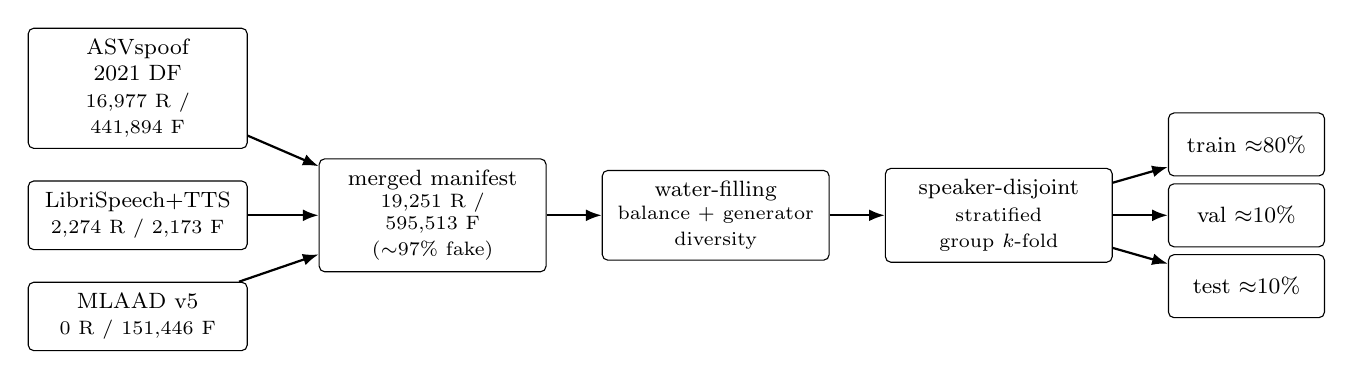
\begin{tikzpicture}[
  node distance=4mm,
  box/.style={draw, rounded corners=2pt, align=center, inner sep=4pt,
              font=\footnotesize, minimum height=8mm, text width=26mm},
  src/.style={box, text width=25mm},
  arr/.style={-{Latex[length=2mm]}, thick}
]
\node[src] (a) {ASVspoof 2021 DF\\\scriptsize 16{,}977 R / 441{,}894 F};
\node[src, below=of a] (b) {Libri\-Speech+TTS\\\scriptsize 2{,}274 R / 2{,}173 F};
\node[src, below=of b] (c) {MLAAD v5\\\scriptsize 0 R / 151{,}446 F};

\node[box, right=9mm of b] (m) {merged manifest\\\scriptsize 19{,}251 R / 595{,}513 F\\\scriptsize ($\sim$97\% fake)};
\node[box, right=7mm of m] (w) {water-filling\\\scriptsize balance + generator\\\scriptsize diversity};
\node[box, right=7mm of w] (s) {speaker-disjoint\\\scriptsize stratified group $k$-fold};

\node[box, right=7mm of s, text width=17mm, yshift=9mm]  (tr) {train $\approx$80\%};
\node[box, right=7mm of s, text width=17mm]              (va) {val $\approx$10\%};
\node[box, right=7mm of s, text width=17mm, yshift=-9mm] (te) {test $\approx$10\%};

\draw[arr] (a) -- (m); \draw[arr] (b) -- (m); \draw[arr] (c) -- (m);
\draw[arr] (m) -- (w); \draw[arr] (w) -- (s);
\draw[arr] (s) -- (tr); \draw[arr] (s) -- (va); \draw[arr] (s) -- (te);
\end{tikzpicture}}
\caption{Benchmark construction. Three public corpora are merged into one
labelled manifest, reduced to a class-balanced and generator-diverse subset of
19{,}251\,+\,19{,}251 clips by the water-filling allocation of
Algorithm~\ref{alg:waterfill}, then partitioned so that no speaker or synthesis
voice crosses a boundary. R = real, F = fake.}
\label{fig:pipeline}
\end{figure}

\subsection{Signal preprocessing}\label{sec:preproc}

Audio is decoded (see Sect.~\ref{sec:hygiene}), mixed to mono, resampled to
16\,kHz, and fixed to 4\,s (64{,}000 samples) by zero-padding short clips and
cropping long ones---randomly during training, centred at evaluation. Log-mel
spectrograms use 80 mel bands with a 400-sample window (25\,ms) and a 160-sample
hop (10\,ms), giving an $80 \times 401$ representation per clip. The classical
baseline instead takes 40 MFCCs from the same front-end
settings~\cite{torchaudio}.

% =====================================================================
\section{Data hygiene: a silent decoder failure}\label{sec:hygiene}
% =====================================================================

Building the benchmark surfaced a failure mode that we report in full because it
is silent, class-correlated, and invisible to every metric in this paper.

\paragraph{The failure}
The \texttt{soundfile} Python binding to \texttt{libsndfile} fails to decode a
large fraction of the ASVspoof~2021 DF FLAC files, reporting a decoder
synchronisation error, even though the files are valid and decode correctly with
FFmpeg. In our first pipeline the affected reads did not propagate as
exceptions to the caller: they produced empty or zero-valued waveforms, which the
fixed-length preprocessing step (Sect.~\ref{sec:preproc}) then padded to 4\,s of
digital silence.

We quantify the failure exactly rather than estimating it. Re-running
\texttt{libsndfile} alone over the 38{,}502-clip benchmark manifest and counting
the clips that either raise or return all-zero audio gives
Table~\ref{tab:decoder}. Almost half the ASVspoof real partition
(8{,}456 of 16{,}977 clips, 49.8\%) and a comparable share of its fake partition
(3{,}613 of 8{,}539, 42.3\%) fail; the LibriSpeech+TTS and MLAAD sources are
unaffected at exactly zero failures. With the FFmpeg fallback in place the
count over the same manifest is $0$ of $38{,}502$.

\begin{table}[t]
\centering
\caption{Clips that \texttt{libsndfile} alone fails to decode, or decodes to
all-zero audio, over the balanced benchmark manifest. The failure is confined to
ASVspoof~2021~DF and is roughly class-neutral \emph{within} that corpus; the
class asymmetry in the last two rows is induced at benchmark level, because
ASVspoof supplies 88\% of the benchmark's real audio but only 44\% of its fake
audio. With the FFmpeg fallback enabled every count in this table becomes zero.}
\label{tab:decoder}
\small\setlength{\tabcolsep}{5pt}
\begin{tabular}{@{}llrrr@{}}
\toprule
Source & Class & Failed & Total & Rate (\%) \\
\midrule
ASVspoof~2021~DF   & real & 8{,}456 & 16{,}977 & 49.8 \\
ASVspoof~2021~DF   & fake & 3{,}613 &  8{,}539 & 42.3 \\
LibriSpeech+TTS    & real &       0 &  2{,}274 &  0.0 \\
LibriSpeech+TTS    & fake &       0 &  2{,}173 &  0.0 \\
MLAAD~v5           & fake &       0 &  8{,}539 &  0.0 \\
\midrule
\textbf{All}       & \textbf{real} & \textbf{8{,}456} & \textbf{19{,}251} & \textbf{43.9} \\
\textbf{All}       & \textbf{fake} & \textbf{3{,}613} & \textbf{19{,}251} & \textbf{18.8} \\
\bottomrule
\end{tabular}
\end{table}

\paragraph{Why it is worse than random corruption}
The corruption is not distributed uniformly over the benchmark. Within ASVspoof
the failure rate is similar for both classes (49.8\% real, 42.3\% fake), so the
decoder itself is not class-selective. The asymmetry is a property of the
\emph{merge}: ASVspoof is the only source contributing a large quantity of
\emph{real} speech, so at benchmark level 43.9\% of real clips are silenced
against 18.8\% of fake clips---a 2.3$\times$ imbalance---and the silent clips
fall predominantly in the real class. A model presented with this data has
an exact, trivially learnable rule available---all-zero input implies
real---which is far easier than any spectral cue. It is a textbook
shortcut~\cite{shortcut}: perfectly predictive on the corrupted training
distribution, and worthless on any correctly decoded input.

\paragraph{Why aggregate metrics do not catch it}
The validation and test partitions are decoded by the same broken path, so they
carry the same shortcut. EER, balanced accuracy, ROC-AUC, and the per-class
report are all computed on a distribution in which the shortcut is valid, and
all of them look healthy. There is no aggregate number in this paper---or in a
typical anti-spoofing results table---that would have exposed it. The same
argument applies to any silent, deterministic, class-correlated preprocessing
failure, of which decoder incompatibility is only the instance we happened to
hit.

\paragraph{Detection and fix}
The detection procedure is cheap and we recommend it as a routine step: after
decoding, compute per-clip signal energy over the whole manifest and cross-tabulate
the count of all-zero or near-zero clips against \texttt{label} and
\texttt{dataset\_source}. A healthy corpus gives a small, class-independent
count; a decoder failure gives a large count concentrated in one
(source, label) cell. The fix is a fallback decoder: attempt
\texttt{soundfile} first for speed, and on any exception fall back to
FFmpeg~\cite{ffmpeg}, which reads the affected files correctly. Every number
reported in this paper is post-fix, and Table~\ref{tab:decoder} is the
cross-tabulation the procedure produces.

One implementation detail is worth recording, because it caused the bug to
recur silently after it had once been fixed. Our fallback originally called
librosa~\cite{librosa}, which wraps FFmpeg. librosa was later removed from the
pinned environment for an unrelated dependency conflict, but an empty
\texttt{librosa/} directory was left in \texttt{site-packages}; under Python's
implicit-namespace-package rule this directory still satisfies
\texttt{import librosa}. The import therefore succeeded, the attribute lookup on
it failed at call time, and that failure was absorbed by the same
zero-on-exception handler described below---reinstating the exact shortcut the
fallback existed to prevent, with no error surfaced. The lesson generalises
beyond this package: a fallback path that is only exercised on the failure
branch of a \texttt{try} block is never exercised in normal testing, so its own
availability must be asserted at start-up rather than assumed. We now resolve
the FFmpeg binary explicitly at import and fail loudly if it is absent.

A related subtlety affects the classical baseline. Its feature extractor
returned an all-zero MFCC vector for any file it could not read, mirroring the
same failure into the classical arm. Silent zero-filling on error is convenient
for keeping a batch pipeline running and dangerous for exactly this reason: a
per-file failure becomes a per-class feature. Where robustness to unreadable
files is genuinely required, the count of such files should be reported.

% =====================================================================
\section{Detectors}\label{sec:methods}
% =====================================================================

\subsection{Reproducing the classical pipeline}\label{sec:classical}

We reproduce the audited pipeline~\cite{unmasking} on our benchmark. Forty MFCCs
are computed per clip with the front-end settings of Sect.~\ref{sec:preproc} and
summarised over time by their mean and standard deviation, giving an
80-dimensional vector per clip, standardised before classification. Two feature
sets are evaluated per classifier, mirroring the audited paper's own comparison:

\begin{itemize}
\item \textbf{MFCC}: the 80-dimensional summary vector directly.
\item \textbf{GNB+NMF transfer}: the 18-dimensional representation described in
Sect.~\ref{sec:degenerate}---two GNB class posteriors concatenated with a
16-component NMF decomposition of the MFCC features. The NMF is fitted on
min-max-scaled training features only (NMF requires non-negative input), and
transform-time features are clipped at zero, since test values can fall slightly
outside the training range.
\end{itemize}

Four classifiers are evaluated on each: Gaussian Naive Bayes (the audited
paper's headline configuration), logistic regression, a random forest (50 trees,
maximum depth 10), and $k$-nearest neighbours ($k = 5$)~\cite{sklearn}. All
transforms are fitted on the training partition only.

\subsection{AttentiveSpecCNN}\label{sec:model}

The proposed detector replaces the audited pipeline's static
MFCC\,$\rightarrow$\,GNB\,$\rightarrow$\,NMF chain with a learned,
frame-weighted representation. It is deliberately small: 106{,}149 parameters,
trainable in minutes on a single consumer GPU.

An input log-mel spectrogram $X \in \mathbb{R}^{1 \times 80 \times 401}$ is first
passed through a batch-normalisation layer that maps raw decibel values (roughly
$-100$ to $+40$) to a stable range. Four convolutional blocks follow, with
channel widths 16, 32, 64, and 128; each block is a $3\times3$ convolution,
batch normalisation, ReLU, and $2\times2$ max-pooling. The output is a feature
map $F \in \mathbb{R}^{128 \times 5 \times 25}$.

The frequency axis is collapsed by averaging, giving a sequence
$H = (\mathbf{h}_1, \dots, \mathbf{h}_T) \in \mathbb{R}^{128 \times T}$ with
$T = 25$. Because four stride-2 poolings downsample time by a factor of 16 from
a 10\,ms hop, each of these $T$ positions advances by 160\,ms of audio; this sets
the temporal resolution of the explanations in Sect.~\ref{sec:explain}.

Temporal attention pooling then computes a scalar score per frame with a learned
linear map $\mathbf{w} \in \mathbb{R}^{128}$, $b \in \mathbb{R}$, normalises the
scores over time, and forms a context vector as the weighted mean:
\begin{equation}
\alpha_t = \frac{\exp(\mathbf{w}^\top \mathbf{h}_t + b)}
                {\sum_{t'=1}^{T} \exp(\mathbf{w}^\top \mathbf{h}_{t'} + b)},
\qquad
\mathbf{c} = \sum_{t=1}^{T} \alpha_t \, \mathbf{h}_t .
\label{eq:attn}
\end{equation}
The context vector is classified by a two-layer head
($128 \rightarrow 64$, ReLU, dropout 0.3, $64 \rightarrow 2$) whose output
columns are ordered $[\text{real}, \text{fake}]$.

Equation~\eqref{eq:attn} is the substantive departure from the audited pipeline.
Where that pipeline applies a fixed transform to a fixed summary statistic---the
MFCC mean and standard deviation over the whole clip, which weights every frame
equally---the attention layer \emph{learns} how much each moment of audio
contributes to the real/fake decision, and does so as part of the detection
objective rather than as a separate unsupervised preprocessing step. Attention
pooling of this form is established in speaker embedding~\cite{attnpool}; its
role here is as a learned generalisation of the audited feature engineering, and
as an explanation channel.

Table~\ref{tab:config} gives the full configuration.

\begin{table}[t]
\centering
\caption{Audio front-end, model, and training configuration for AttentiveSpecCNN.}
\label{tab:config}
\begin{tabular}{@{}lp{0.58\columnwidth}@{}}
\toprule
Setting & Value \\
\midrule
Sample rate / channels & 16\,kHz, mono \\
Clip length            & 4\,s (64{,}000 samples); pad if short, else random crop (train) / centre crop (eval) \\
Log-mel spectrogram    & 80 mel bands, $n_\text{fft}{=}400$, hop${=}160$ $\rightarrow$ $80{\times}401$ \\
Input normalisation    & BatchNorm over the single input channel \\
CNN backbone           & 4 blocks, channels 16/32/64/128, $3{\times}3$ conv + BN + ReLU + $2{\times}2$ max-pool \\
Pooling                & frequency mean, then temporal attention (Eq.~\eqref{eq:attn}), $T{=}25$ frames at 160\,ms \\
Classifier head        & Linear $128{\to}64$, ReLU, dropout 0.3, Linear $64{\to}2$ \\
Parameters             & 106{,}149 \\
Optimiser / schedule   & Adam, lr $10^{-3}$, ReduceLROnPlateau ($\times 0.5$, patience 2) \\
Loss                   & cross-entropy with inverse-frequency class weights \\
Batch size / epochs    & 64 / 15, checkpoint selected by best validation EER \\
Hardware               & single NVIDIA RTX 3080 \\
\bottomrule
\end{tabular}
\end{table}

\subsection{Explainability}\label{sec:explain}

Two explanation views come out of the architecture without additional
machinery.

The \textbf{attention weights} $\alpha_t$ of Eq.~\eqref{eq:attn} are a per-frame
importance curve read directly off the pooling layer---not a post-hoc
attribution, but the actual quantity the model uses to weight evidence over
time. At 160\,ms resolution over a 4\,s clip they localise the decision to
specific moments: onsets, silences, and transitions.

\textbf{Grad-CAM}~\cite{gradcam} over the final convolutional block supplies the
complementary time--frequency view. Writing $F^{(k)}$ for the $k$-th channel of
the final feature map and $y^{c}$ for the logit of the predicted class $c$, the
channel weights and localisation map are
\begin{equation}
\beta^c_k = \frac{1}{|F^{(k)}|}\sum_{i,j} \frac{\partial y^c}{\partial F^{(k)}_{ij}},
\qquad
L^c = \mathrm{ReLU}\!\left(\sum_k \beta^c_k F^{(k)}\right),
\end{equation}
with $L^c$ max-normalised and bilinearly upsampled to the input
$80 \times 401$ grid. The two views answer different questions---\emph{when} the
model looked, and \emph{where in the time--frequency plane} the evidence
was---and Sect.~\ref{sec:explainres} reads them together.

% =====================================================================
\section{Evaluation protocol}\label{sec:protocol}
% =====================================================================

Every method in this paper is trained on the same speaker-disjoint training
partition and evaluated on the same held-out test partition, with the
validation partition used only for checkpoint and schedule decisions.

We report \textbf{Equal Error Rate} as the primary metric: the operating point
at which the false-acceptance and false-rejection rates coincide, computed from
the receiver operating characteristic over $P(\text{fake})$ scores. EER is
threshold-free and therefore immune to the class-collapse failure of
mechanism M3. Alongside it we report \textbf{balanced accuracy} at the 0.5
threshold, \textbf{per-class F1}, and \textbf{ROC-AUC}. Balanced accuracy and
per-class F1 are included specifically so that a collapse to a single predicted
class is visible rather than hidden; ROC-AUC is included because it is the most
robust of the four under the fixed-threshold, single-run conditions of the
cross-dataset probe (Sect.~\ref{sec:loso}).

Reported figures are single runs at a fixed seed (42), with one exception: the
protocol-inflation ablation of Sect.~\ref{sec:leakage} runs five seeds and
reports mean\,$\pm$\,s.d., because its entire claim is that a number
\emph{moves} between protocols, and that movement must be separated from seed
noise. We state the distinction plainly rather than implying more;
Sect.~\ref{sec:limits} discusses what each does and does not license.

% =====================================================================
\section{Results}\label{sec:results}
% =====================================================================

\subsection{In-domain detection}\label{sec:indomain}

Table~\ref{tab:indomain} and Fig.~\ref{fig:method} report all nine
configurations on the same speaker-disjoint test partition.

\begin{table}[t]
\centering
\caption{In-domain detection on the speaker-disjoint test partition; lower EER
is better. GNB+NMF denotes the audited paper's 18-dimensional ``transfer''
representation (Sect.~\ref{sec:degenerate}); $\dagger$ marks its headline
configuration. The proposed model roughly halves the best classical
configuration's EER, and the audited headline is the weakest of the nine.}
\label{tab:indomain}
\small\setlength{\tabcolsep}{4.5pt}
\begin{tabular}{@{}llrrrr@{}}
\toprule
Method & Features & EER (\%) & Bal.\ acc.\ (\%) & F1$_{\text{fake}}$ (\%) & AUC \\
\midrule
\textbf{AttentiveSpecCNN (ours)} & log-mel & \textbf{4.81}  & \textbf{93.84} & \textbf{93.49} & \textbf{0.99} \\
Random Forest          & MFCC    & 11.33 & 87.51 & 87.86 & 0.96 \\
Random Forest          & GNB+NMF & 11.89 & 87.60 & 87.83 & 0.95 \\
$k$-Nearest Neighbours & MFCC    & 13.15 & 85.46 & 86.13 & 0.92 \\
Logistic Regression    & GNB+NMF & 14.78 & 84.73 & 84.09 & 0.92 \\
$k$-Nearest Neighbours & GNB+NMF & 15.05 & 83.93 & 84.67 & 0.91 \\
Logistic Regression    & MFCC    & 15.52 & 84.33 & 84.17 & 0.91 \\
Gaussian Naive Bayes   & GNB+NMF & 23.93 & 76.72 & 75.77 & 0.87 \\
Gaussian Naive Bayes$^{\dagger}$ & MFCC & 26.69 & 73.05 & 71.75 & 0.81 \\
\bottomrule
\end{tabular}
\end{table}

\begin{figure}[t]
\centering
\safefig{\columnwidth}{fig_method_comparison.png}
\caption{Equal Error Rate by method on the speaker-disjoint test partition. The
proposed AttentiveSpecCNN roughly halves the EER of the best classical
configuration.}
\label{fig:method}
\end{figure}

Three readings follow.

First, the audited pipeline's \emph{best} configuration on an honest protocol is
a random forest over raw MFCCs at 11.33\% EER. That is a respectable classical
result; it is not 99.93\% accuracy, and the gap between the two is the
combined contribution of mechanisms M1--M4.

Second, the audited pipeline's \emph{headline} configuration---Gaussian Naive
Bayes over MFCCs---is the worst of the nine, at 26.69\% EER and 0.81 AUC.
The configuration the original work promotes is not the configuration its own
feature set supports best, which is consistent with a selection driven by
accuracy under leakage rather than by detection ability.

Third, AttentiveSpecCNN reaches 4.81\% EER, a 57.5\% relative reduction from
11.33\%, at 106{,}149 parameters. Balanced accuracy (93.84\%) and
F1$_{\text{fake}}$ (93.49\%) are close to each other and to accuracy, which
confirms that the improvement is genuine two-class separation rather than a
shift in the collapse direction.

\subsection{Does the GNB+NMF transfer step help?}\label{sec:transfer}

Table~\ref{tab:indomain} answers the audited paper's central methodological
claim directly, and the answer is no. Pairing each classifier with itself across
the two feature sets:

\begin{itemize}
\item Random forest: $11.33 \rightarrow 11.89$\% EER (transfer is \emph{worse}).
\item $k$-nearest neighbours: $13.15 \rightarrow 15.05$\% EER (worse).
\item Logistic regression: $15.52 \rightarrow 14.78$\% EER (better by 0.74).
\item Gaussian Naive Bayes: $26.69 \rightarrow 23.93$\% EER (better by 2.76).
\end{itemize}

The step helps the two weakest classifiers and hurts the two strongest,
including the best configuration overall. This is the signature of a
dimensionality-reduction step, not of feature enrichment: compressing 80
dimensions to 18 regularises a high-bias model (Gaussian Naive Bayes, whose
conditional-independence assumption is badly violated by correlated cepstral
coefficients) and discards usable variance for a low-bias one (the random
forest). It does not add information, because---as Sect.~\ref{sec:degenerate}
argues---there is no additional information for it to add: the GNB posteriors
are a deterministic function of the same MFCCs the NMF sees.

We report this as a negative result on the audited method's stated contribution.
Its classifiers work; its feature-refinement step does not earn its place.

\subsection{Explainability}\label{sec:explainres}

Figure~\ref{fig:explain} shows the two explanation views for a correctly
identified real clip: the input log-mel spectrogram, the Grad-CAM map over the
time--frequency plane, and the temporal attention curve $\alpha_t$.

\begin{figure}[t]
\centering
\safefig{0.95\columnwidth}{fig_explain.png}
\caption{Explanation for a correctly identified real clip. Top: input log-mel
spectrogram. Middle: Grad-CAM over the final convolutional block, showing which
time--frequency regions supported the predicted class. Bottom: the temporal
attention weights $\alpha_t$ of Eq.~\eqref{eq:attn}---25 values at 160\,ms
spacing, linearly interpolated onto the input frame axis for display.}
\label{fig:explain}
\end{figure}

The attention curve is non-uniform, which is the first thing worth checking: a
model that had learned to ignore the time axis would produce a flat
$\alpha_t \approx 1/T$ and the pooling layer would reduce to a mean, making the
architecture equivalent to global average pooling. It does not. Mass
concentrates on voiced regions and on transitions into and out of them, and
the Grad-CAM map concentrates in the corresponding columns, so the two views
agree about \emph{when} even though they are computed by different mechanisms
(a forward-pass weight versus a backward-pass gradient attribution).

We are deliberate about what this does and does not establish. It establishes
that the model's decision is temporally localised and that the localisation is
consistent across two independent views---which is what an operator auditing a
flagged clip needs. It does not establish that the highlighted regions contain
the \emph{synthesis artefact}, and Sect.~\ref{sec:loso} gives a concrete reason
for scepticism: a model that is partly reading recording domain will produce
confident, well-localised, internally consistent explanations of a cue that has
nothing to do with synthesis. Explanation fidelity and explanation
\emph{correctness} are different properties, and only the first is demonstrated
here.

\subsection{Cross-dataset generalisation}\label{sec:loso}

The in-domain protocol of Sect.~\ref{sec:benchmark} removes mechanisms M1--M3
but not M4: training and test partitions still draw on the same three sources.
To measure M4, we hold out an entire source. For each held-out source, a fresh
AttentiveSpecCNN is trained on the other two---rebalanced by the same
water-filling allocation---and evaluated on the held-out one
(Table~\ref{tab:cross}, Fig.~\ref{fig:cross}).

\begin{table}[t]
\centering
\caption{Leave-one-source-out generalisation. MLAAD contributes no real audio,
so when it is held out only the fake-detection rate on unseen generators is
reportable. The in-domain row is the reference point from
Table~\ref{tab:indomain}.}
\label{tab:cross}
\small\setlength{\tabcolsep}{5pt}
\begin{tabular}{@{}lllr@{}}
\toprule
Held-out source & Trained on & Metric & Result \\
\midrule
\emph{(reference) in-domain} & all three  & EER / AUC   & \textbf{4.81\% / 0.99} \\
ASVspoof 2021 (DF)           & LS+TTS, MLAAD & EER / AUC & 44.93\% / 0.56 \\
LibriSpeech + TTS            & ASVspoof, MLAAD & EER / AUC & 57.50\% / 0.42 \\
MLAAD v5                     & ASVspoof, LS+TTS & fake-recall & 48.4\% \\
\bottomrule
\end{tabular}
\end{table}

\begin{figure}[t]
\centering
\safefig{\columnwidth}{fig_cross_dataset.png}
\caption{In-domain versus held-out ROC-AUC. Performance collapses to, or below,
chance when the test source is entirely unseen during training.}
\label{fig:cross}
\end{figure}

Performance collapses. A detector at 4.81\% EER and 0.99 AUC in-domain reaches
0.56 AUC on unseen ASVspoof audio and 48.4\% recall on unseen MLAAD
generators---both indistinguishable from a coin flip. Whatever supports the
in-domain result is largely not present in a new source.

The Libri\-Speech+TTS fold is more informative than the others, because 0.42 AUC
is not merely chance---it is \emph{below} chance, which means the ranking is
systematically inverted and therefore carries real, anti-correlated signal. The
mechanism is visible in the training composition. That fold trains on ASVspoof
(telephone-band, codec-degraded, containing most of the real audio) and MLAAD
(clean, wideband, entirely fake). Across those two sources, acoustic
cleanliness is almost perfectly predictive of the label---clean implies
fake---and it is a far easier cue than any synthesis artefact. The held-out
Libri\-Speech+TTS real speech is clean studio audiobook audio, so the learned rule
assigns it to ``fake'' with confidence. The detector did not fail to learn; it
learned a corpus-polarity rule that happens to be exactly wrong on the held-out
source. This is shortcut learning~\cite{shortcut} with an unusually clean
diagnosis, and it is the strongest single piece of evidence in this paper that
the in-domain 4.81\% figure leans on recording-domain signature.

Two asymmetries qualify the numbers. The ASVspoof-holdout fold is real-starved:
with ASVspoof removed, the only real speech available for training is the
$\sim$2.3k clips of the Libri\-Speech+TTS set, so that row should be read as a
lower bound rather than a clean measurement. And MLAAD's fake-only composition means
the MLAAD row measures generator generalisation alone, with no real-class
component. Neither asymmetry changes the direction of the result, and both are
properties of the available public data rather than of the protocol.

% =====================================================================
\section{Discussion}\label{sec:discussion}
% =====================================================================

\subsection{What the 99.93\% figure measures}\label{sec:whatitmeasures}

The audited result is best understood not as an error but as a correct
measurement of the wrong quantity. Under mechanisms M1 and M2, a substantial
part of the test partition is recoverable from the training partition---by
interpolation for the synthetic minority points, and by speaker identity for the
rest. A high-capacity classifier that memorises the training partition
therefore scores well on the test partition, and accuracy (M3) reports that
score without exposing the class-collapse configurations underneath. What was
measured is the pipeline's ability to reproduce its own training data. That
ability is real; it is simply not deepfake detection.

The corrected figure on our benchmark is 11.33\% EER for the best configuration
of the same method family. We emphasise that this is not a small number to be
embarrassed about---a classical MFCC pipeline at 11\% EER on a merged,
speaker-disjoint, three-corpus benchmark is a reasonable classical baseline.
The problem was never the method's capability; it was the protocol's inability
to measure it.

\subsection{The in-domain result is also partly domain signature}\label{sec:ourown}

Intellectual consistency requires applying the audit to our own headline number.
The 4.81\% EER of Sect.~\ref{sec:indomain} is free of mechanisms M1--M3 by
construction, but it is not free of M4, and Sect.~\ref{sec:loso} quantifies how
much that matters: on a fully unseen source the same architecture is at
chance. The correct reading of 4.81\% is therefore ``on a merged
three-corpus benchmark with speaker-disjoint partitions'', with the qualifier
carrying real weight. The one thing the leave-one-source-out study licenses us
to say is that any single-corpus number, including a properly split one, should
be assumed non-transferable until it is tested across corpora.

\subsection{A reporting checklist}\label{sec:checklist}

The mechanisms in Sect.~\ref{sec:audit} recur widely enough that we state the
corresponding checks compactly. For an audio deepfake detection result reported
on an ad-hoc or merged corpus:

\begin{enumerate}
\item \textbf{Report EER}, not accuracy alone. If accuracy is reported, report
per-class recall beside it so class collapse is visible.
\item \textbf{Split on speaker, not on rows.} State the grouping variable and how
it was derived per source. Assert disjointness programmatically.
\item \textbf{Resample, if at all, inside the training partition only.} Prefer
subsampling the majority class or class-weighted losses to synthesising minority
points~\cite{smote}, and state which was used.
\item \textbf{State the class ratio} of the corpus before any balancing, so the
majority-class baseline can be computed by the reader.
\item \textbf{State the generator composition} of the fake class. A fake class
dominated by one generator measures one generator.
\item \textbf{Audit the decoder.} Cross-tabulate near-zero-energy clip counts by
label and source before training (Sect.~\ref{sec:hygiene}). Report the count of
unreadable files rather than zero-filling silently, and assert at start-up that
any fallback decoder is actually callable---a fallback is only exercised on the
failure branch, so its own absence is invisible to normal testing.
\item \textbf{Report at least one cross-corpus number.} An in-domain result
without one bounds nothing about deployment.
\item \textbf{Verify that a proposed component earns its place} by an ablation
against its own absence, per classifier---not only in the configuration where it
happens to help (Sect.~\ref{sec:transfer}).
\end{enumerate}

\subsection{Relation to companion work}\label{sec:companion}

The generalisation gap measured in Sect.~\ref{sec:loso} is a diagnosis, not a
remedy, and this paper deliberately stops at the diagnosis. A companion study by
the same authors~\cite{companion}, under review elsewhere, addresses the remedy
with unsupervised test-time adaptation of self-supervised detectors. The two
works are disjoint in every experimental respect: they use different corpora
(ASVspoof~2019~LA, In-the-Wild, and an Arabic set there; ASVspoof~2021~DF, the
Libri\-Speech+TTS set, and MLAAD here), different detector families
(fine-tuned XLS-R there; classical MFCC pipelines and a 106k-parameter CNN
here), and different claims. No table, figure, or reported number is shared. We
declare the relationship here so that the scope of each is unambiguous to
readers and editors.

\subsection{Limitations}\label{sec:limits}

\paragraph{MLAAD contributes no real audio}
The most consequential property of the benchmark
(Sect.~\ref{sec:sources}). Every MLAAD clip in the training set carries a
source-identity signal correlated with the label, so part of the in-domain
separation in Table~\ref{tab:indomain} is source discrimination rather than
deepfake detection. This is why Sect.~\ref{sec:loso} exists; it is measured
rather than assumed. A benchmark with real audio from every source would be
better and does not currently exist in the public multilingual TTS setting.

\paragraph{Single-run results}
All figures are single runs at seed 42, except the protocol-inflation ablation
(Sect.~\ref{sec:leakage}), which is run over five seeds. We therefore do not claim
statistical significance for any comparison in Table~\ref{tab:indomain}, and small
differences there---notably the 0.74-point logistic-regression gain in
Sect.~\ref{sec:transfer}---should be read as within the range that seed variation
could plausibly produce. The two conclusions we do draw from that table are
larger than any plausible seed effect: the 6.5-point gap between
AttentiveSpecCNN and the best classical configuration, and the ranking of the
audited headline configuration as last.

\paragraph{The real-starved ASVspoof fold}
Discussed in Sect.~\ref{sec:loso}: that row is a lower bound.

\paragraph{Fixed-threshold cross-dataset probes}
The cross-dataset numbers are single-run and evaluated at a fixed threshold, for
which ROC-AUC is the most robust of the reported statistics; the EER values in
Table~\ref{tab:cross} should be read as accompanying detail rather than as
precisely estimated quantities.

\paragraph{Scope of the explainability claim}
Established in Sect.~\ref{sec:explainres}: explanation fidelity is demonstrated,
explanation correctness is not.

\paragraph{The audited paper's corpus}
We reproduce the audited \emph{method} on our benchmark rather than re-running
the audited \emph{evaluation} on its original corpus. The audit in
Sect.~\ref{sec:audit} therefore rests on the protocol as described in that
paper and on structural argument for the corpus it was run on, not on a
re-execution of it there. Sect.~\ref{sec:leakage} instead re-runs our own
benchmark under progressively leakier protocols and measures M2's contribution
directly (a matched-pair, 5-seed +10.4-point accuracy / $-$10.4-point EER
movement from splitting randomly instead of by speaker); M1's marginal
contribution on top of M2 is not cleanly isolated by that design, for the
reason given there, and is left to an arm that holds pool composition fixed
across the resampling/no-resampling comparison.

% =====================================================================
\section{Conclusion}\label{sec:conclusion}
% =====================================================================

An implausibly high published accuracy for audio deepfake detection turns out to
be the correct output of an evaluation that measures memorisation rather than
detection, through four independent and compounding mechanisms: pre-split
oversampling, random folding over a speaker-recurrent corpus, accuracy as the
headline metric, and a single fixed recording domain. The method's advertised
feature-refinement step is additionally degenerate as specified, and does not
help on an honest protocol---it worsens the strongest classical model.

On a merged, class-balanced, generator-diverse, speaker-disjoint benchmark built
from three public corpora, the same method family reaches 11.33\% EER, and a
compact 106{,}149-parameter attention CNN reaches 4.81\% EER while supplying
per-frame attention and Grad-CAM explanations at no extra cost. That in-domain
result then fails to transfer: on a fully unseen source, ROC-AUC falls to 0.56
and, in one direction, to 0.42, which we trace to a corpus-polarity shortcut in
which acoustic cleanliness rather than synthesis artefact carries the decision.

We also document a silent decoder failure that turns roughly half of one
corpus's audio into digital silence, concentrated in one class, producing a
shortcut that no aggregate metric in this paper would have exposed. Reporting it
is not incidental to the argument: it is the same argument at the level of the
data pipeline rather than the protocol. In both cases the number looked fine and
the measurement was not.

The open problem in this field is not headline accuracy. It is robust
generalisation, and honest measurement of it.

% =====================================================================
\backmatter

\bmhead{Acknowledgements}
The authors thank Manipal University Jaipur for supporting this work. We thank
the maintainers of the ASVspoof, LibriSpeech, and MLAAD corpora for releasing
the data that made this study possible.

\section*{Declarations}

\bmhead{Availability of data and materials}
All three source corpora are publicly available: ASVspoof~2021~\cite{asvspoof21},
LibriSpeech~\cite{librispeech}, and MLAAD~v5~\cite{mlaad}. The code that builds
the merged manifest, draws the class-balanced subset, produces the
speaker-disjoint splits, reproduces the classical baseline, and trains and
explains AttentiveSpecCNN is released at
\url{https://github.com/RohamIzadidoost/Kaggle_deepFakeAudio},
together with the manifest-construction scripts needed to regenerate the exact
benchmark from the public sources.

\bmhead{Competing interests}
The authors declare that they have no competing interests.

\bmhead{Funding}
This research received no specific grant from any funding agency in the public,
commercial, or not-for-profit sectors. The article-processing charge is covered
by Manipal University Jaipur.

\bmhead{Authors' contributions}
R.I. designed and implemented the benchmark construction, the detectors, and all
experiments, and drafted the manuscript. S.S. (Sumit Srivastava) supervised the
work, contributed to the study design and the evaluation protocol, and revised
the manuscript. S.S. (Shweta Sharma) contributed to the experimental design and
the analysis, and revised the manuscript. All authors read and approved the
final manuscript.

\bmhead{Ethics approval and consent to participate}
Not applicable. This study uses only publicly released speech corpora and
involves no human participants recruited by the authors.

\bmhead{Consent for publication}
Not applicable.

\bibliography{refs_jasmp}

\end{document}
